\documentclass[9pt,twocolumn,twoside]{osajnl}
\journal{ol} % Choose journal (ao, aop, josaa, josab, ol, pr)
% See template introduction for guidance on setting shortarticle option
\setboolean{shortarticle}{true}
% \documentclass[11pt,twocolumn,twoside]{osajnl}
\usepackage{caption,graphicx,subcaption,overpic,tikz,tkz-tab,verbatim,multirow,booktabs,siunitx,amsmath,amssymb,bm,mathtools,threeparttable,color,enumitem,listingsutf8,url,xcolor,etaremune,bibentry,textcomp,mathpazo,geometry,lastpage,fancyhdr,float,epstopdf,bm,upgreek}
\usepackage{lineno}
\linenumbers


\newcommand{\op}[1]{\ensuremath{\mathcal{#1}}}

%%%%%%%%%%%%%%%%%%%%%%%%%%%%%%%%%%%%%%%%%%%%%%%%%%%%%%%%%%%%%%%%%%%%
\title{Volumetric imaging by complex holographic deconvolution}

\author[1]{Ni Chen}
\author[2]{Peng Xia}
\author[3]{Edmund Y. Lam}
\author[1,*]{Byoungho Lee}


\affil[1]{Department of Electrical and Computer Engineering,
Seoul National University, Seoul 08826, Korea}
\affil[2]{xxxxxxxxxxxxxxxxxxxxxxxxxxxx, Japan}
\affil[3]{Department of Electrical and Electronic Engineering, The University of Hong Kong, Pokfulam, Hong Kong}

\affil[*]{Corresponding author: byoungho@snu.ac.kr}

%% To be edited by editor
% \dates{Compiled \today}

%\ociscodes{(140.3490) Lasers, distributed feedback; (060.2420) Fibers, polarization-maintaining;(060.3735) Fiber Bragg gratings.}

%% To be edited by editor
% \doi{\url{http://dx.doi.org/10.1364/XX.XX.XXXXXX}}

\graphicspath{{./figure/}}

\begin{abstract}
We propose a volumetric imaging through three-dimensional holographic deconvolution approach. Both simulation and experimental results show our method works perfectly for overlapped objects with continues and discrete depth.

\end{abstract}

\setboolean{displaycopyright}{true}

\begin{document}

\maketitle

\section{Introduction}\label{sec_intro}
Holography is a regarded as a perfect technique for both three-dimensional~(3D) imaging~\cite{Chen2018Sensors} and display~\cite{Hong2011AO}, because it contains the object wavefront.
The original holography are based on the interference of object wave and reference wave, which record the object wavefront into an intensity image. The interferometric holography induces DC term, twin image problem.
There are various techniques that can obtain the complex wavefront of the object wave, Among different configurations for recording the holographic information of an object, in this Letter we focus
on optical scanning holography (OSH) [12,13] and the
Mach–Zehnder interferometer-based DH [14,15]. 
such as optical scanning holography~(OSH)~\cite{Poon2009JOSK} and phase-shift holography~(PSH)~\cite{Yamaguchi2008OaPN}.

Digital holography (DH) is a unique imaging technique that
can record the whole wavefront information, including amplitude and phase, of a three-dimensional (3D) specimen in a
noninvasive way. With a two-dimensional (2D) hologram,
one can achieve optical sectioning [1], extended focused imaging [2], 3D imaging [3], etc.

Even though holography records the 3D information, it hardly been used for imaging compared to other techniques. 
when we reconstruct holograms digitally, we usually reconstruct plane images along the optical axis. The 3D information other than the focused one induces defocus noises, which usually hindered the useful information. Sectional reconstruction is used to resolve this problem. 
There were many research published. However no one reconstruct a whole 3D volume, especially for overlapped objects. 
To our best acknowledge, this is the first that can reconstruct a totally overlapped 3D objects.

In DH microscopy, an important step is to obtain an individual object section from a 3D object, a process known as sectioning or sectional image reconstruction. The conventional method for sectioning in OSH uses the conjugate of the system impulse response, but the main drawback is that a large residue signal from the undesired object section remains, which is often called the defocus noise. To improve this, methods using Wiener filter ~\cite{Kim2006AO}, Wigner distribution~\cite{Kim2008AO}, and inverse imaging~\cite{Lam2009AO,Zhang2010JOSA} have been developed.

\section{Method}\label{sec_method}
Suppose $r=(x,y)$, when an 3D object $o(r,z)$ is illuminated by a plane wave, the result object wavefront at a point of $(r_h, z_h)$ can be represented as a convolution of the object function with the impulse response of free-space propagation~\cite{Goodman2005}
\begin{equation}
\begin{aligned}
u(r_h,z_h) 
& = \iiint o(r,z) \frac{\exp(jk\sqrt{(r_h-r)^2 + (z_h-z)^2})}{\sqrt{(r_h-r)^2 + (z_h-z)^2}} d r dz, \\
& = o(r,z) \otimes \frac{\exp(jk\sqrt{r^2 + z^2})}{\sqrt{r^2 + z^2}},
\label{eq_3ddiffr}
\end{aligned}
\end{equation}
where $k$ is the wave number, $\otimes$ is the convolution operator, and $h(r,z)=\frac{\exp(jk\sqrt{r^2 + z^2})}{\sqrt{r^2 + z^2}}$ is the point spread function~(PSF). 
Both OSH and PSH can obtain the object wavefront directly or indirectly.
The digital reconstruction, thus can be obtained by back-propagation of the  wavefront $u(r_h,z_h)$. The complex conjugate $h^*(r, z_r)$ is used to convolve with the hologram to reconstruct the section at the corresponding position
\begin{equation}
\begin{aligned}
o^\prime(r,z_r) 
& = u(r_h,z_h)\otimes h^*(r,z_r) \delta(z_r-z_h) , \\
& = o(r,z_r)\vert_{z_r=z_h} + o(r,z_r) \otimes h(r, z_h) \otimes h^*(r,z_r) \vert_{z_r \neq z_h}
\label{eq_3ddiffr_inv}
\end{aligned}
\end{equation}
It is clear that the reconstructed section contains an unwanted second term, which act as noise, and usually submerges the object signal, especially for a complex 3D object. 



Eq.~(\ref{eq_3ddiffr}) can be written as a linear transformation
\begin{equation}
\Im\left\{u(r,z_h)\right\} = \Im\left\{o(r,z)\right\} \Im\left\{h(r,z)\right\} \label{eq_3dholo_ft}
\end{equation}
We represent the lexicographically ordered 2D hologram $\Im\left\{u(r,z)\right\}$ as a vector of $\mathbf{U(z)}$. 
Similarly, $\Im\left\{o(r,z)\right\}$ is represented as a vector $\mathbf{O}(r,z)$ . $\Im\left\{h(r,z)\right\}$ is represented as $\mathbf{H}(k_r, z)$.
The product of $\Im\left\{o(x,y,z)\right\} \mathbf{H}(k_x,k_y,k_z)$ becomes $\mathbf{H}(r,z)\mathbf{O}(r,z)$.
Because of the complexity property of the holography, we write Eq.~(\ref{eq_3dholo_ft}) as
\begin{equation}
\begin{bmatrix}
\mathbf{U}_R \\ \mathbf{U}_I 
\end{bmatrix}
=\begin{bmatrix}
H_R(z_1) & \dots & H_R(z_n) \\
H_I(z_1) & \dots & H_I(z_n) 
\end{bmatrix}
\begin{bmatrix}
\mathbf{O}_R(z_1) & \mathbf{O}_I(z_1)\\ 
\vdots  & \vdots \\
\mathbf{O}_R(z_n) & \mathbf{O}_I(z_n) \\  
\end{bmatrix}
\end{equation}

% \begin{equation}
% \begin{bmatrix}
% \mathbf{g}_R \\ 
% \mathbf{g}_I 
% \end{bmatrix}
% =\begin{bmatrix}
% H_R(z_1) \\ \dots \\ H_R(z_n) \\
% H_I(z_1) \\ \dots \\ H_I(z_n) 
% \end{bmatrix}^\intercal
% \begin{bmatrix}
% \mathbf{o}_R(z_1) \\ 
% \vdots \\
% \mathbf{o}_R(z_n) \\ 
% \mathbf{o}_I(z_1) \\
% \vdots  \\
% \mathbf{o}_I(z_n)
% \end{bmatrix}
% \end{equation}


This is an inverse problem under convex, non-smooth regularizes, the unconstrained form is
\begin{equation}
\mathbf{O}_{est} = \min_\mathbf{O} \frac{1}{2} \lVert \mathbf{H}\mathbf{O} - \mathbf{G} \rVert _2^2  + \tau \phi(\mathbf{O})
\label{eq_3dholo}
\end{equation}
where $\tau \in R_+$ is the regularization parameter.



%
%Algorithms can be included using the commands as shown in algorithm \ref{alg:euclid}.
%
%\begin{algorithm}
%\caption{Euclid’s algorithm}\label{alg:euclid}
%\begin{algorithmic}[1]
%\Procedure{Euclid}{$a,b$}\Comment{The g.c.d. of a and b}
%\State $r\gets a\bmod b$
%\While{$r\not=0$}\Comment{We have the answer if r is 0}
%\State $a\gets b$
%\State $b\gets r$
%\State $r\gets a\bmod b$
%\EndWhile\label{euclidendwhile}
%\State \textbf{return} $b$\Comment{The gcd is b}
%\EndProcedure
%\end{algorithmic}
%\end{algorithm}

\section{Results}\label{sec_results}

Figure \ref{fig_sim} shows the simulation results. 
Several objects of various 3D structures with their side and top views shown in Fig.~\ref{fig_sim}(a) were used to verify the feasibility of our method. The colorbar show the transmittance of the object. The left object, which is a helix function, has no overlapping along the optics. The center one, which is consist of three geometric shapes, has partially overlapping, and the right one, which is a circular helix, is totally overlapped. 
Fig.~\ref{fig_sim}(b) shows the holograms of each of the object in Fig.~\ref{fig_sim}(a). In the hologram calculation process, Gaussian noise was added.
Fig.~\ref{fig_sim}(c) are the reconstructions with back propagation. The signals are totally hided in the reconstructed volume.
Fig.~\ref{fig_sim}(d) is the results use our method. Which shows the 3D object clearly. It should be mentioned that both the partially and totally overlapped information were reconstructed perfectly.

\begin{figure*}[htbp]
\centering

\begin{minipage}[b]{1\textwidth}
\centering
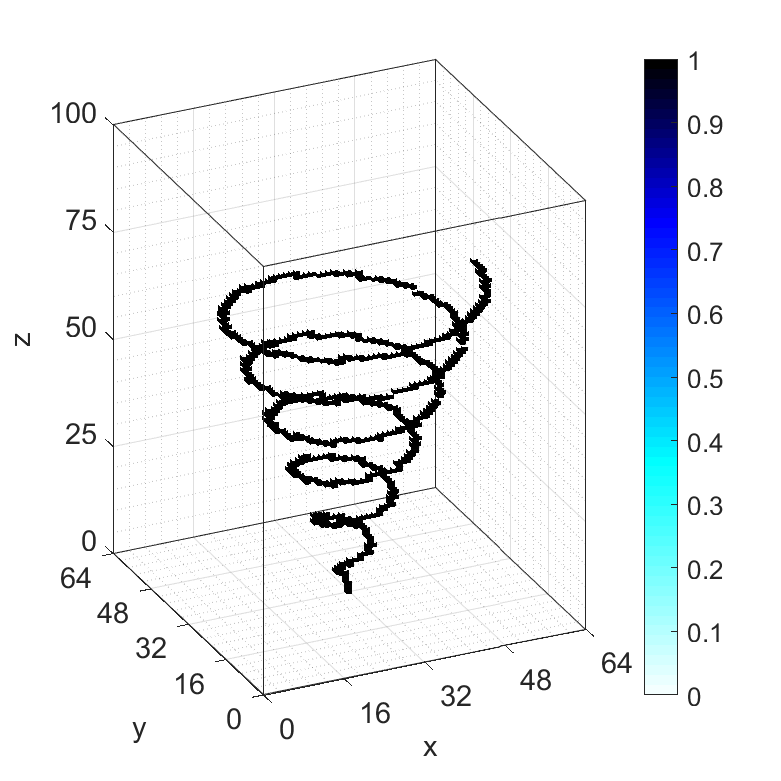
\includegraphics[width=0.18\columnwidth]{conhelix}
\begin{subfigure}[b]{0.18\textwidth}
  \centering
  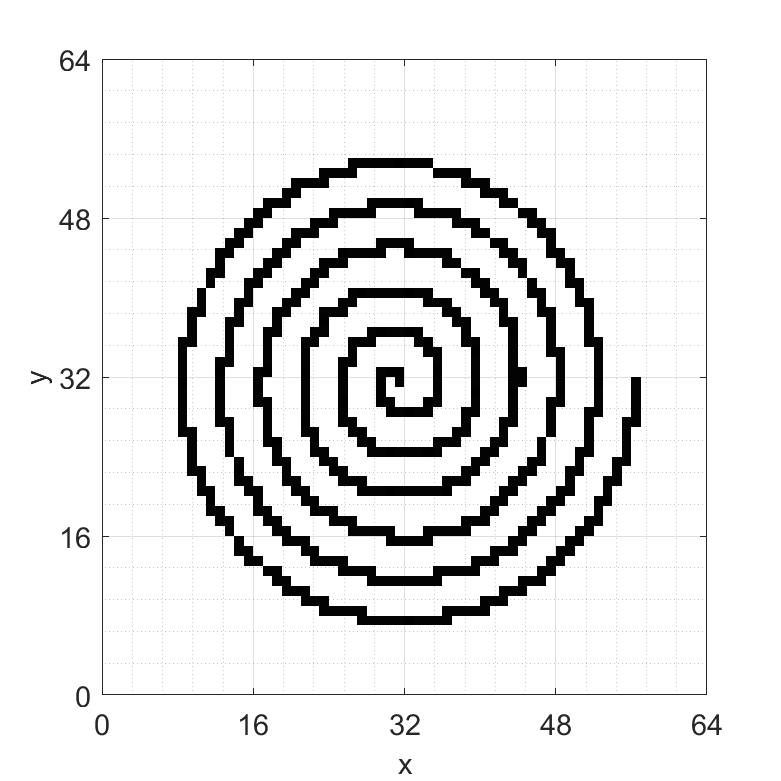
\includegraphics[width=0.45\columnwidth]{conhelix_top}

  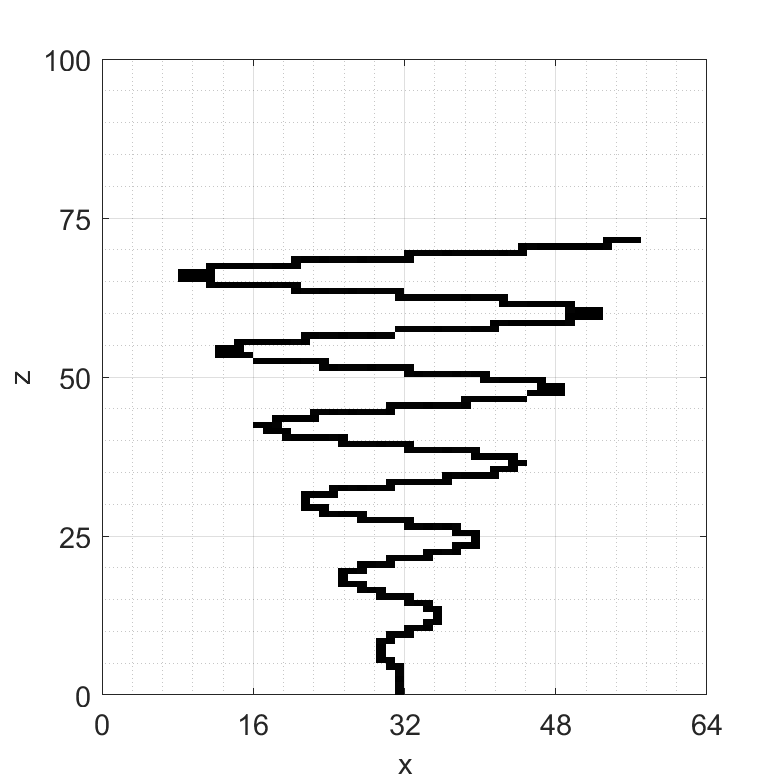
\includegraphics[width=0.45\columnwidth]{conhelix_side}
\end{subfigure}
\begin{subfigure}[b]{0.18\textwidth}
  \centering
  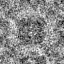
\includegraphics[width=0.45\columnwidth]{conhelix_complex_holo}

  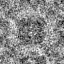
\includegraphics[width=0.45\columnwidth]{conhelix_complex_holo}
\end{subfigure}
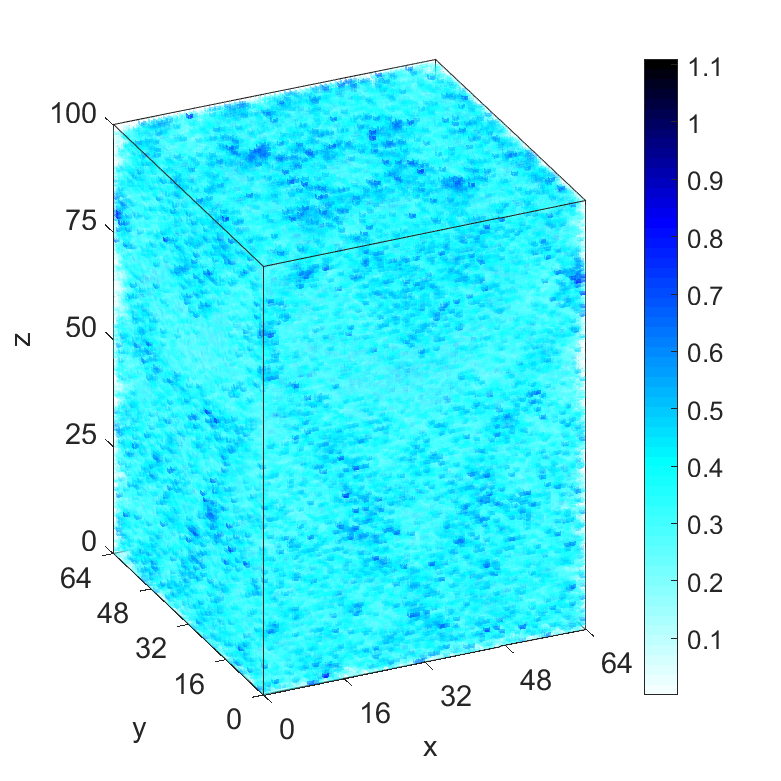
\includegraphics[width=0.18\textwidth]{conhelix_complex_BP_3d}
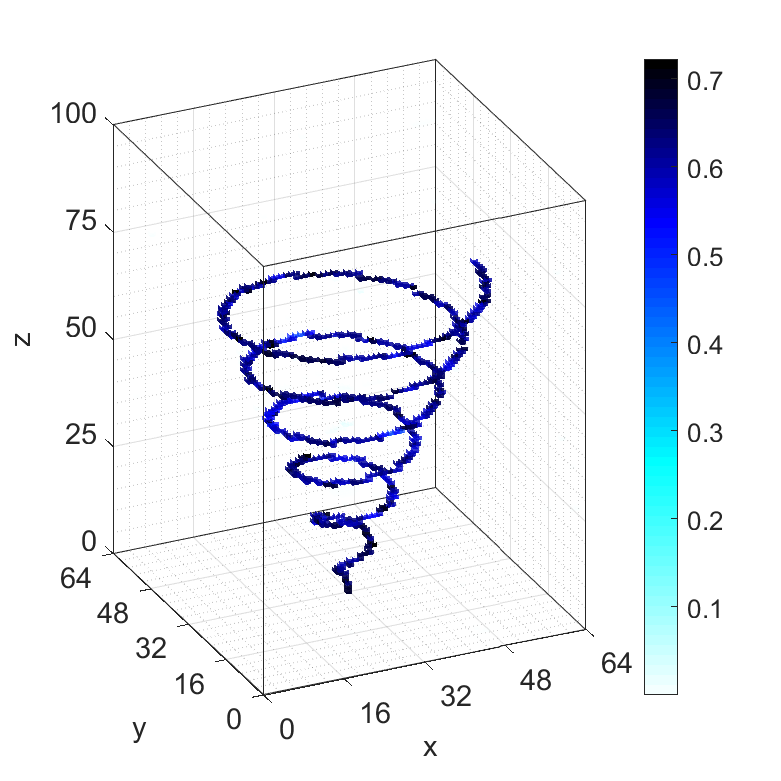
\includegraphics[width=0.18\textwidth]{conhelix_complex_TwIST_3d}
\subcaption{}
\end{minipage}

\begin{minipage}[b]{1\textwidth}
\centering
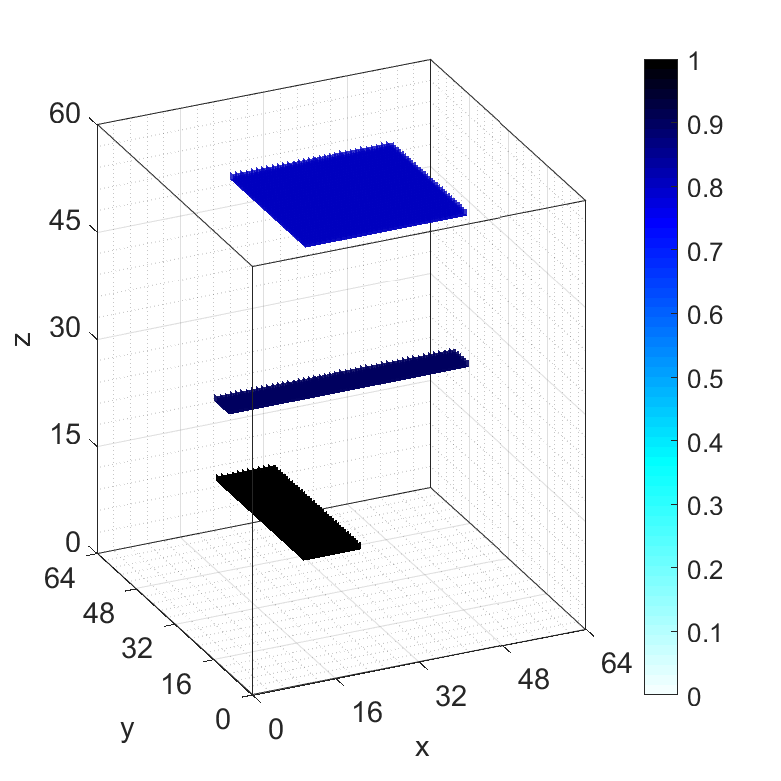
\includegraphics[width=0.18\columnwidth]{overlap}
\begin{subfigure}[b]{0.18\textwidth}
  \centering
  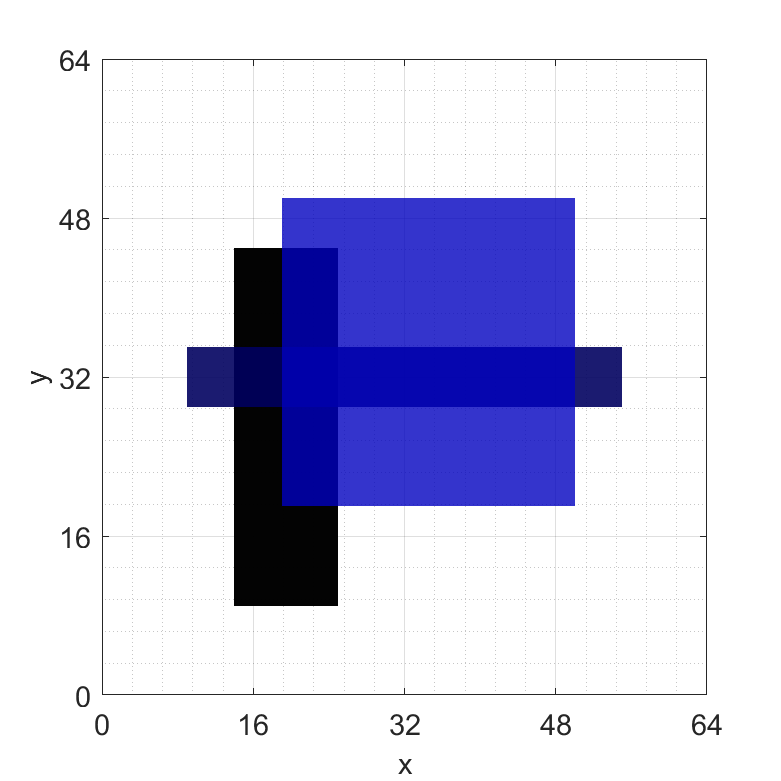
\includegraphics[width=0.45\columnwidth]{overlap_top}

  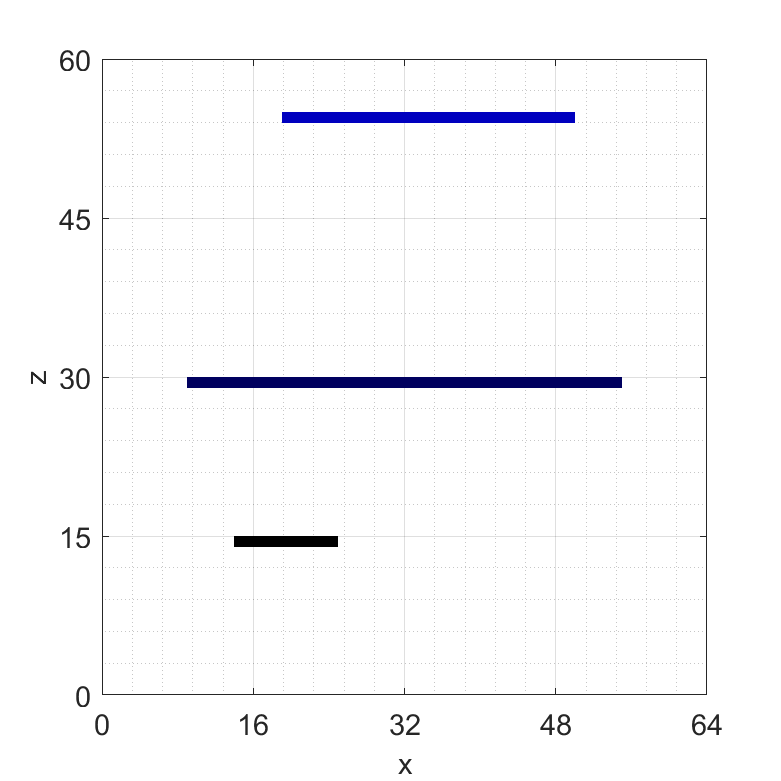
\includegraphics[width=0.45\columnwidth]{overlap_side}
\end{subfigure}
\begin{subfigure}[b]{0.18\textwidth}
  \centering
  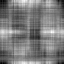
\includegraphics[width=0.45\columnwidth]{overlap_complex_holo}

  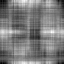
\includegraphics[width=0.45\columnwidth]{overlap_complex_holo}
\end{subfigure}
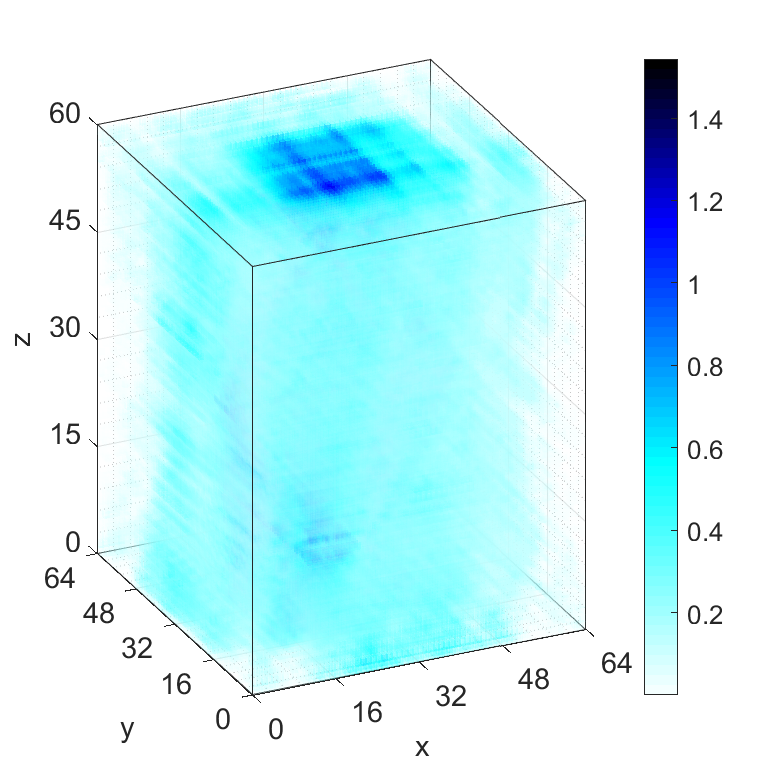
\includegraphics[width=0.18\textwidth]{overlap_complex_BP_3d}
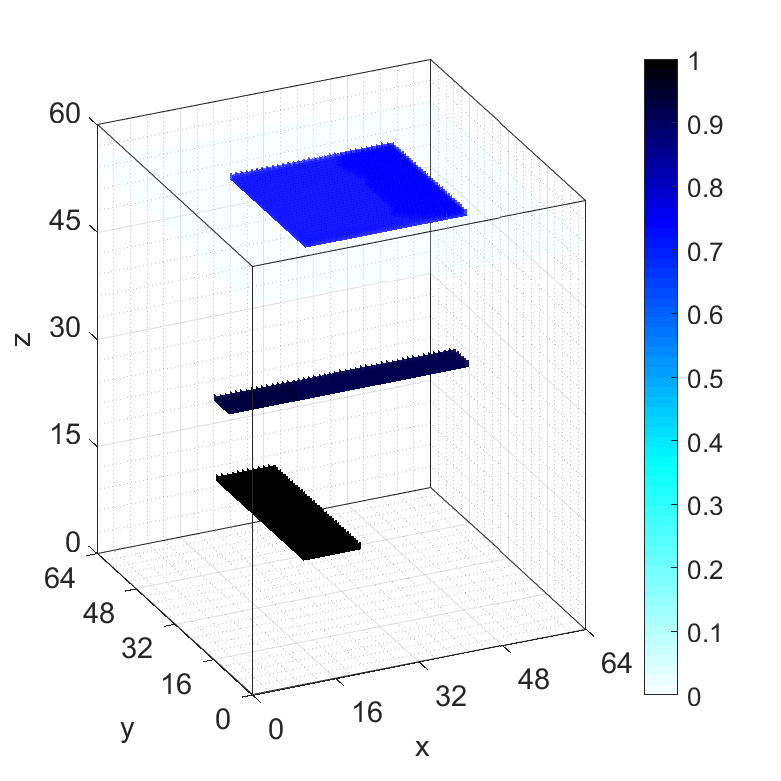
\includegraphics[width=0.18\textwidth]{overlap_complex_TwIST_3d}
\subcaption{}
\end{minipage}

\begin{minipage}[b]{1\textwidth}
\centering
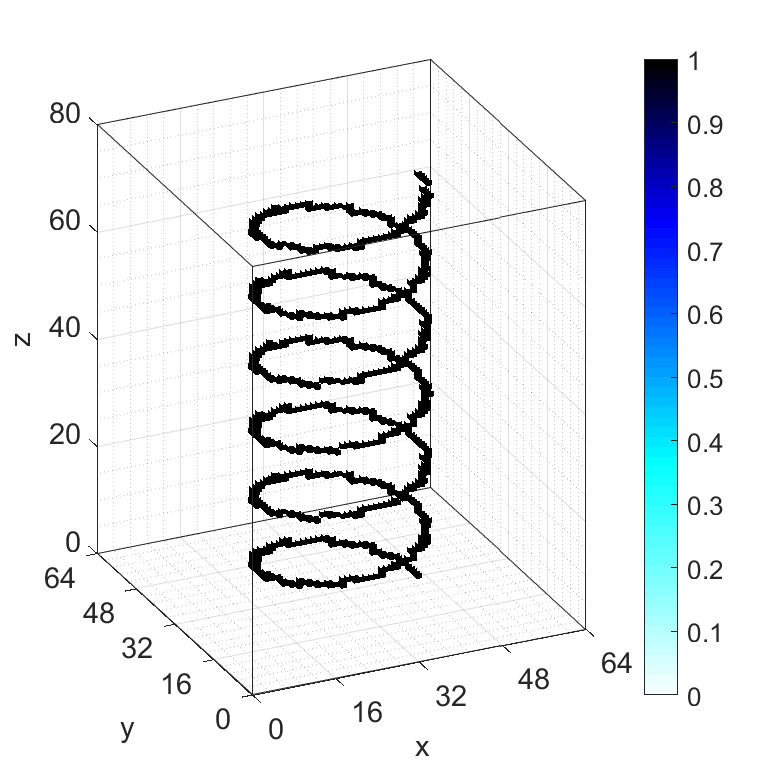
\includegraphics[width=0.18\columnwidth]{cirhelix}
\begin{subfigure}[b]{0.18\textwidth}
  \centering
  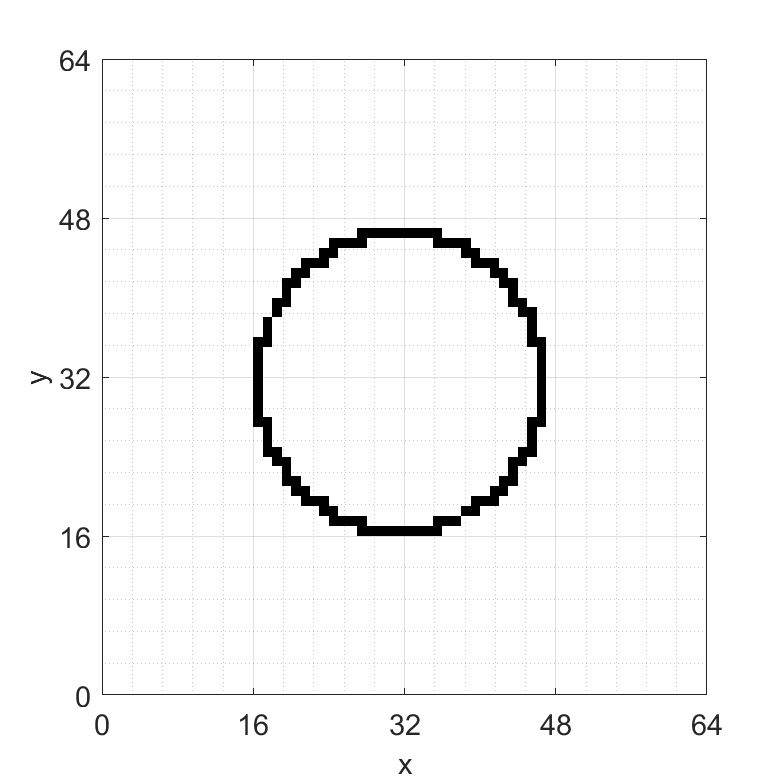
\includegraphics[width=0.45\columnwidth]{cirhelix_top}

  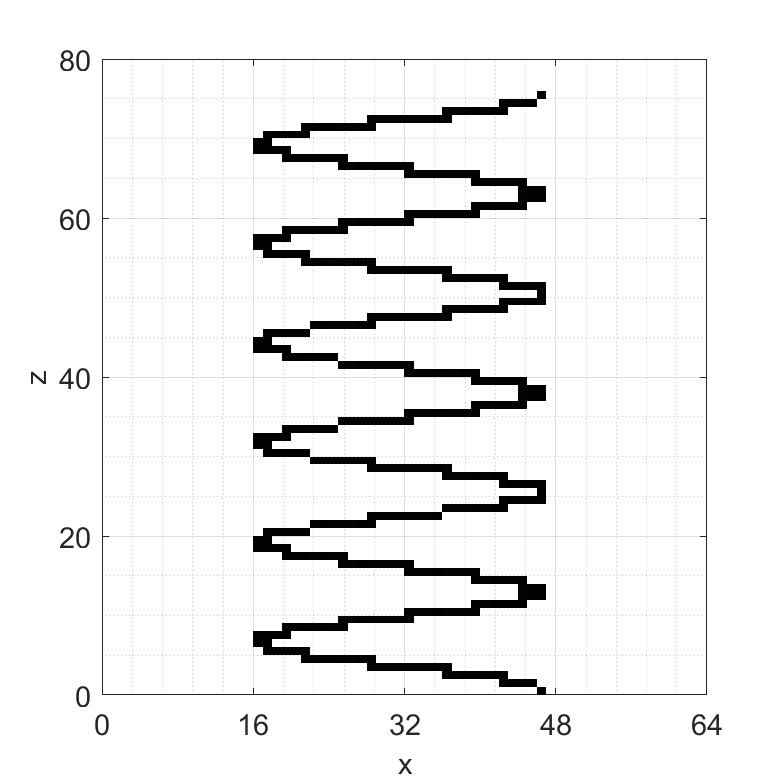
\includegraphics[width=0.45\columnwidth]{cirhelix_side}
\end{subfigure}
\begin{subfigure}[b]{0.18\textwidth}
  \centering
  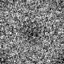
\includegraphics[width=0.45\columnwidth]{cirhelix_complex_holo}

  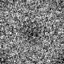
\includegraphics[width=0.45\columnwidth]{cirhelix_complex_holo}
\end{subfigure}
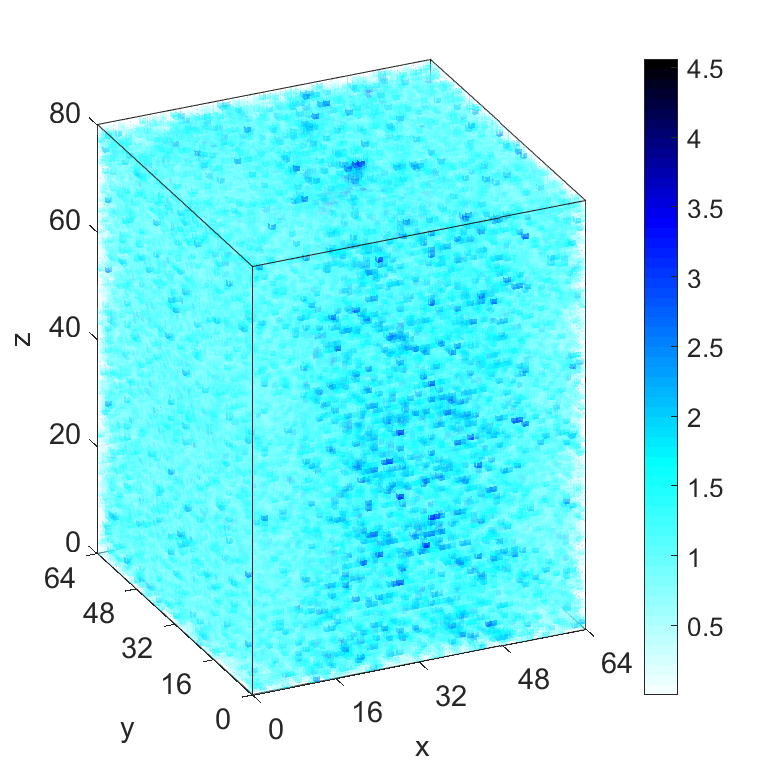
\includegraphics[width=0.18\textwidth]{cirhelix_complex_BP_3d}
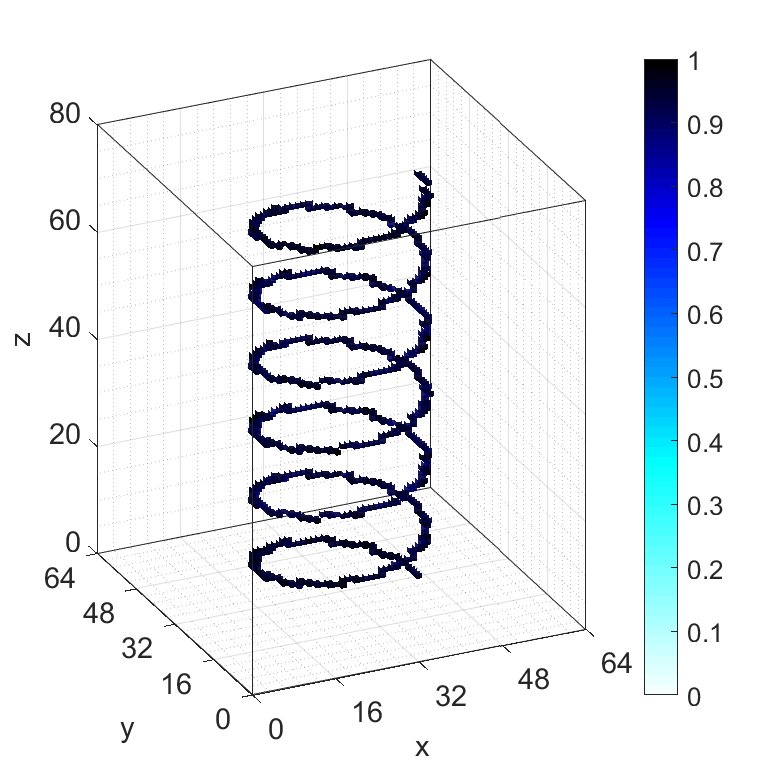
\includegraphics[width=0.18\textwidth]{cirhelix_complex_TwIST_3d}
\subcaption{}
\end{minipage}
\caption{Simulation (Gaussian noise with 35db)}
\label{fig_sim}
\end{figure*}

% \begin{table}[htbp]
% \centering
% \caption{\bf Shape Functions for Quadratic Line Elements}
% \begin{tabular}{ccc}
% \hline
% local node & $\{N\}_m$ & $\{\Phi_i\}_m$ $(i=x,y,z)$ \\
% \hline
% $m = 1$ & $L_1(2L_1-1)$ & $\Phi_{i1}$ \\
% $m = 2$ & $L_2(2L_2-1)$ & $\Phi_{i2}$ \\
% $m = 3$ & $L_3=4L_1L_2$ & $\Phi_{i3}$ \\
% \hline
% \end{tabular}
% \label{tab:shape-functions}
% \end{table}


\section{Funding}

Brain Korea Plus 2019; National Science Foundation of China (NSFC) (61705241).

% The authors thank H. Haase, C. Wiede, and J. Gabler for technical support.

%%%%%%%%%%%%%%%%%%%%%%%%%%%%%%%%%%%%%%%%%%%%%%%%%%%%%%%%%%%%%%%%%
\bibliography{3dholoref}

\bibliographyfullrefs{3dholoref}

\end{document}
